\section{Types of Random Variables}

Random variables are classified based on the type of probability measure they induce on the real line. Formally, this measure is defined on the \textbf{Borel $\sigma$-algebra}, the collection of all sets that we consider \textit{measurable} on the real line. Now, it turns out that there are three fundamentally distinct ways a probability measure can behave on the real line. An important result in measure theory, known as the \textbf{Lebesgue Decomposition Theorem} (we will see this theorem later), guarantees that any probability measure on $\mathbb{R}$ can be uniquely expressed as a combination of these three types of measures. These foundational types are Discrete, Continuous and Singular. Thus, we say that there are three \textit{pure type} random variables, namely: \textbf{discrete random variables}, \textbf{continuous random variables}, and \textbf{singular random variables}. Furthermore, it is possible to construct random variables by combining these pure types, resulting in what we call \textbf{mixed random variables}. In total, this yields seven possible types of random variables, including these mixtures.\\

However, for most applications—especially in engineering and statistics—only \textbf{discrete} and \textbf{continuous random variables} are practically significant. \textbf{Singular random variables} are rarely encountered outside of theoretical discussions and are mostly studied in academia. Consequently, our primary focus will be on understanding discrete and continuous random variables, though we will also define and illustrate an example of a singular random variable for completeness.\\

\subsection{Discrete Random Variables}

\begin{definition}
    A random variable \( X \) is called \textit{discrete} if it takes values in a countable subset of \( \mathbb{R} \) with probability 1. In other words, there exists a countable set \( E = \{ x_1, x_2, \dots \} \) such that \( P_X(E) = 1 \), meaning the entire probability distribution of \( X \) is contained within this set. 
\end{definition}

To clarify, we don’t necessarily require that the \textit{range} of \( X \) itself is countable; only that \( X \) almost surely takes values in a countable subset. There may still be some subset of the sample space that maps to an uncountable subset of \( \mathbb{R} \) but with probability zero.\\

\begin{definition}
    Given a discrete random variable \( X \), we define the function \( p_X: \mathbb{R} \to [0, 1] \) by
\[
p_X(x) = P(X = x) \quad \text{for every } x.
\]
This function \( p_X \) is called the \textit{probability mass function} (PMF) of \( X \). While \( p_X(x) \) is defined for all \( x \in \mathbb{R} \), it’s important to observe that \( p_X(x) \) is only non-zero for \( x \in E \), the countable set where \( X \) has probability mass.
\end{definition}

Since \( P_X(E) = 1 \), the additivity property of probabilities implies:
\[
\sum_{i=1}^{\infty} P(X = x_i) = 1.
\]

This summation states that the total probability across all possible values \( X \) can take must equal 1.\\

For a discrete random variable \( X \), the PMF \( p_X \) alone provides a complete description of the probability distribution of \( X \). For any Borel set \( B \subset \mathbb{R} \), we can determine the probability that \( X \) falls within \( B \) by summing over the values in \( E \) that are also in \( B \):
\[
P_X(B) = \sum_{i : x_i \in B} P(X = x_i).
\]

This relation highlights that for any subset \( B \) of the real numbers, we only need to consider the countable values where the PMF is non-zero.\\

For a discrete random variable, the cumulative distribution function (CDF) \( F_X \) at any point \( x \) is given by the sum of probabilities for all values \( x_i \leq x \):
\[
F_X(x) = \sum_{i : x_i \leq x} P(X = x_i).
\]
This CDF describes the probability that \( X \) takes a value less than or equal to \( x \), accumulated over all points in \( E \) up to \( x \).\\

To illustrate some of the most common discrete random variables, we delve into a few key examples below, each defined on a probability space \((\Omega, \mathcal{F}, P)\).\\

\textbf{1. Indicator Random Variable:}\\

Let \( A \in \mathcal{F} \) be any event. We define the indicator random variable \( I_A : \Omega \to \{0,1\} \) by
\[
I_A(\omega) = 
\begin{cases} 
1, & \text{if } \omega \in A, \\
0, & \text{if } \omega \notin A.
\end{cases}
\]
The variable \( I_A \) is indeed a random variable because both \( A \) and \( A^c \) are \(\mathcal{F}\)-measurable. As it only takes two values (0 and 1), it is clearly discrete.\\

\textbf{2. Bernoulli Random Variable:} \\

Consider a parameter \( p \in [0, 1] \). We define a random variable \( X \) with probability mass function (PMF) given by
\[
P(X = 0) = p \quad \text{and} \quad P(X = 1) = 1 - p.
\]
This random variable can represent a single coin toss: \( X = 0 \) can signify \textit{heads} with probability \( p \), and \( X = 1 \) can represent \textit{tails} with probability \( 1 - p \). If \( p = \frac{1}{2} \), the coin is fair.\\


\textbf{3. Discrete Uniform Random Variable:}  \\

Suppose \( a \) and \( b \) are integers with \( a < b \). Define a random variable \( X \) with values \( m = a, a+1, \dots, b \) and probability
\[
P(X = m) = \frac{1}{b - a + 1}.
\]
This variable takes each integer between \( a \) and \( b \) inclusively with equal probability. Outside this range, \( P(X = m) = 0 \).\\

\textbf{4. Binomial Random Variable:} \\

Given a parameter \( p \in [0, 1] \) and an integer \( n \in \mathbb{N} \), a binomial random variable \( X \) counts the number of successes in \( n \) independent trials, each with success probability \( p \). Its PMF is
\[
P(X = k) = \binom{n}{k} p^k (1 - p)^{n - k} \quad \text{for } k = 0, 1, \dots, n.
\]
This model applies to scenarios like counting the number of heads in \( n \) independent coin tosses with success probability \( p \).\\

\textbf{5. Geometric Random Variable:}  \\

For \( 0 < p \leq 1 \), the geometric random variable \( X \) represents the number of independent trials required to obtain the first success. Its PMF is given by
\[
P(X = k) = p (1 - p)^{k - 1} \quad \text{for } k = 1, 2, \dots
\]
This model could describe, for instance, the number of coin tosses until the first head appears, where each toss has a success probability of \( p \).\\

\textbf{6. Poisson Random Variable:}  \\

Given a parameter \( \lambda > 0 \), a Poisson random variable \( X \) represents the number of occurrences of an event in a fixed interval, assuming events occur with a constant mean rate \( \lambda \). The PMF of \( X \) is
\[
P(X = k) = \frac{e^{-\lambda} \lambda^k}{k!} \quad \text{for } k = 0, 1, 2, \dots
\]
The Poisson model is often used for count data, such as the number of emails received per hour.\\

Except for the indicator random variable, each of these examples is primarily defined by its PMF rather than an explicit mapping from the sample space \( \Omega \). 

\subsection{Continuous Random Variables}

To properly define continuous random variables, we need to understand the concept of \textbf{absolute continuity} between measures.

\begin{definition}
    Let \(\mu\) and \(\nu\) be measures on \((\Omega, \mathcal{F})\). We say that \(\nu\) is \textit{absolutely continuous} with respect to \(\mu\) if for every set \(N \in \mathcal{F}\) where \(\mu(N) = 0\), we also have \(\nu(N) = 0\). In other words, if \(\mu\) assigns no \textit{weight or size} to \(N\), then \(\nu\) must do the same.
\end{definition}

Now, consider a probability space \((\Omega, \mathcal{F}, P)\) and let \(X : \Omega \to \mathbb{R}\) represent a random variable. We call \(X\) a \textbf{continuous random variable} if the \textit{law} (or distribution) of \(X\), denoted \(P_X\), is absolutely continuous with respect to the \textit{Lebesgue measure} \(\lambda\) on \(\mathbb{R}\).\\

Let’s clarify the terms:\\

(a) The law \(P_X\) is a measure on the real line \((\mathbb{R}, \mathcal{B})\), where \(\mathcal{B}\) is the collection of Borel sets on \(\mathbb{R}\).\\
(b) Absolute continuity of \(P_X\) with respect to \(\lambda\) means that for any Borel set \(N \subseteq \mathbb{R}\) with \(\lambda(N) = 0\), we must also have \(P_X(N) = P(\omega \mid X(\omega) \in N) = 0\).\\

This ensures that a continuous random variable \(X\) does not place probability mass on sets of \textit{Lebesgue measure zero,} such as individual points or countable collections of points.\\

Importantly, just because a random variable \(X\) takes values in an uncountable set does not mean it is continuous. Continuity here is defined in terms of the behavior of the probability measure \(P_X\) in relation to the Lebesgue measure \(\lambda\).\\

To formalize this relationship, we rely on a powerful tool called the \textbf{Radon-Nikodym Theorem}. Though we won’t delve into the proof right now, this theorem asserts that:

\begin{theorem}
    
If \(P_X\) is absolutely continuous with respect to \(\lambda\), there exists a non-negative, measurable function \(f_X\), known as the \textit{Radon-Nikodym derivative} of \(P_X\) with respect to \(\lambda\), such that:
\[
P_X(A) = \int_A f_X(x) \, d\lambda(x)
\]
for any Borel set \(A \subseteq \mathcal{B}(\mathbb{R})\).
\end{theorem}

This function \(f_X\) essentially describes the \textit{density} of the probability measure \(P_X\) relative to \(\lambda\), giving us a precise way to calculate probabilities over continuous random variables.\\

The integral used in the theorem above differs from the typical Riemann integral. This is because the set \( B \) can be any Borel measurable set, such as the Cantor set, not necessarily an interval. In this course, we will later dive into abstract integration to achieve a precise understanding of the integral. For now, however, we can consider \( B \) as a simple interval \([a, b]\).\\

Under this assumption, equation tells us that the probability of the random variable \( X \) falling within the interval \([a, b]\) can be expressed as:
\[
\int_a^b f_X \, dx
\]
where \( f_X \) is a non-negative measurable function.\\

When we say that \( f_X \) is measurable, we mean specifically that if we take the pre-images of Borel sets under \( f_X \), these pre-images are also Borel sets. This property ensures that \( f_X \) is compatible with the Borel structure, making the integration meaningful over any Borel set \( B \). \\

Below, we discuss some prominent examples of continuous random variables, each with unique properties and interpretations.\\

\textbf{1. Uniform Distribution:} \\

The uniform distribution on a closed interval \([a, b]\) is one where each point in the interval has an equal probability density. It is often described as a \textit{scaled Lebesgue measure} over \([a, b]\).\\

(a) \textit{Probability Density Function (PDF)}:
    \[
    f_X(x) = 
    \begin{cases} 
      0 & \text{for } x < a \\
      \frac{1}{b-a} & \text{for } a \leq x \leq b \\
      0 & \text{for } x > b 
   \end{cases}
    \]
    This function shows that outside the interval \([a, b]\), the probability density is zero, and within \([a, b]\), the density is constant.\\

(b) \textit{Cumulative Distribution Function (CDF)}:
    \[
    F_X(x) = 
    \begin{cases} 
      0 & \text{for } x < a \\
      \frac{x - a}{b - a} & \text{for } a \leq x \leq b \\
      1 & \text{for } x > b 
   \end{cases}
    \]
    The CDF \(F_X(x)\) gives the probability that \(X\) is less than or equal to \(x\), increasing linearly within the interval and reaching 1 at \(x = b\).\\

\textbf{2. Exponential Distribution:} \\

The exponential distribution is used to model the time until an event occurs and is defined for \(x \geq 0\), characterized by a parameter \(\lambda > 0\). It is unique in that it has a special property known as the \textbf{memoryless property}.\\

(a) \textit{Probability Density Function (PDF)}:
    \[
    f_X(x) = \lambda e^{-\lambda x} \quad \text{for } x \geq 0
    \]
    Here, \(\lambda\) determines the rate at which probabilities decay as \(x\) increases.\\

(b) \textit{Cumulative Distribution Function (CDF)}:
    \[
    F_X(x) = 1 - e^{-\lambda x} \quad \text{for } x \geq 0
    \]
    This CDF gives the probability that \(X\) is less than or equal to \(x\) and approaches 1 as \(x\) grows, meaning that the event is more likely to have occurred by larger values of \(x\).

\begin{definition}
    \textit{Memoryless Property} states that the probability of an event occurring in the future is independent of the time that has already elapsed. Formally, a non-negative random variable \(X\) is said to be memoryless if:
    \[
    P(X > s + t \mid X > t) = P(X > s) \quad \forall s, t \geq 0.
    \]
\end{definition}


To show that an exponential random variable satisfies this property, consider:
\[
P(X > s + t \mid X > t) = \frac{P((X > s + t) \cap (X > t))}{P(X > t)} = \frac{P(X > s + t)}{P(X > t)}.
\]
Substituting the exponential form, we get:
\[
\frac{e^{-(s+t)\lambda}}{e^{-t\lambda}} = e^{-s\lambda} = P(X > s).
\]
Thus, the exponential distribution indeed possesses the memoryless property. \\

This property has a practical interpretation. For example, if the lifetime of a light bulb is exponentially distributed, then the expected time to failure, given that the bulb has not yet failed by time \(t\), is the same as the expected lifetime of a completely new bulb. Remarkably, the exponential distribution is the only continuous distribution that exhibits this property.\\

\textbf{3. Normal/Gaussian Distribution:} \\

The Gaussian (or Normal) distribution is a fundamental two-parameter distribution, where the parameters are:\\

(a) The mean \(\mu \in \mathbb{R}\), representing the center of the distribution.\\
(b) The standard deviation \(\sigma > 0\), which reflects the spread or dispersion of the distribution.\\

Gaussian distributions are ubiquitous in engineering, statistics, and the natural sciences, largely because they possess a \textit{stable-attractor} property. 

\begin{definition}
    \textit{Stable attractor property} for Gaussian distributions means that sums of independent Gaussian random variables tend to result in a Gaussian distribution.
\end{definition}

This is a major reason for their prominence. We will explore this property and its implications in more detail later.

(a) \textit{Probability Density Function (PDF)}: 
\[
f_X(x) = \frac{1}{\sigma \sqrt{2\pi}} e^{-\frac{(x - \mu)^2}{2\sigma^2}}, \quad x \in \mathbb{R}.
\]
This distribution is commonly denoted as \(N(\mu, \sigma^2)\), where \(\mu\) is the mean and \(\sigma^2\) is the variance (the square of the standard deviation). A particularly notable case occurs when \(\mu = 0\) and \(\sigma^2 = 1\); this is called the \textit{standard Gaussian distribution}, and its PDF simplifies to:
\[
f_X(x) = \frac{1}{\sqrt{2\pi}} e^{-\frac{x^2}{2}}.
\]

(b) \textit{Cumulative Distribution Function (CDF)}: The cumulative distribution function (CDF) of a Gaussian random variable does not have a closed-form expression, which might seem inconvenient. However, this lack of a \textit{closed-form} solution is often manageable and does not detract from its usefulness. For convenience, the CDF of the standard Gaussian (where \(\mu = 0\) and \(\sigma = 1\)) is given a special name: the \textit{error function}, denoted as \(\text{Erf}(x)\), and defined by:
\[
\text{Erf}(x) = \int_{-\infty}^{x} \frac{1}{\sqrt{2\pi}} e^{-\frac{y^2}{2}} \, dy.
\]

This integral essentially captures the probability that a standard Gaussian random variable falls within a particular range, from \(-\infty\) to \(x\), and is widely used in statistics and probability theory.\\

\textbf{4. Cauchy Distribution:} \\

The Cauchy distribution, characterized by two parameters \( x_0 \in \mathbb{R} \) (the location parameter) and \( \gamma > 0 \) (the scale parameter), is a notable example of a \textbf{heavy-tailed} distribution. 

\begin{definition}
    Heavy-tailed nature means that the probability of extreme values does not diminish as rapidly as it would in distributions with lighter tails, like the normal distribution.
\end{definition}

As a result, the Cauchy distribution is commonly used in engineering and other fields to model phenomena with high variability or \textit{burstiness.}\\

(a) \textit{Probability Density Function (PDF)}: 
\[
f_X(x) = \frac{1}{\pi} \frac{\gamma}{(x - x_0)^2 + \gamma^2}.
\]

(b) \textit{Cumulative Distribution Function (CDF)}: To find the cumulative distribution function (CDF) \( F_X(x) \), which represents the probability that \( X \leq x \), we integrate the PDF from \( -\infty \) to \( x \):
\[
F_X(x) = \int_{-\infty}^{x} f_X(t) \, dt = \int_{-\infty}^{x} \frac{1}{\pi} \frac{\gamma}{(t - x_0)^2 + \gamma^2} \, dt.
\]

This integral yields:
\[
F_X(x) = \frac{1}{\pi} \arctan\left( \frac{x - x_0}{\gamma} \right) + \frac{1}{2}.
\]

Thus, the cumulative distribution function of the Cauchy distribution is:
\[
F_X(x) = \frac{1}{\pi} \arctan\left( \frac{x - x_0}{\gamma} \right) + \frac{1}{2}.
\]

This CDF is defined over the entire real line and illustrates the heavy-tailed nature of the Cauchy distribution. Notice that as \( x \to \infty \), \( F_X(x) \to 1 \), while as \( x \to -\infty \), \( F_X(x) \to 0 \), consistent with the fact that this is a probability distribution over \( \mathbb{R} \).

\subsection{Singular Random Variables}

Singular random variables are fascinating and unusual objects in probability theory, often seeming to defy intuition. They are distinct because they exist in a realm that neither discrete nor continuous random variables fully describe. Specifically, singular random variables take on values with probability one within an uncountable set that has a Lebesgue measure of zero. 

\begin{definition}
    A random variable \( X \) is \textbf{singular} if, for any \( x \in \mathbb{R} \), we have \( P_X(\{x\}) = 0 \), and yet there exists a set \( F \in \mathcal{B}(\mathbb{R}) \) (where \( \mathcal{B}(\mathbb{R}) \) denotes the Borel sets on \( \mathbb{R} \)) such that \( F \) has zero Lebesgue measure and \( P_X(F) = 1 \).
\end{definition}

\textit{Why must \( F \) be uncountable?} \\

Suppose \( F \) were countable; then it would only contain a finite or countably infinite number of points, meaning that any random variable with values in \( F \) would be akin to a discrete variable, contradicting our definition of \( P_X(\{x\}) = 0 \) for each \( x \in F \). Therefore, \( F \) must be uncountable, though it still occupies \textit{no space} in terms of Lebesgue measure. \newpage

\textbf{Example: The Cantor Distribution as a Singular Random Variable}\\

An example of a singular random variable arises with the Cantor distribution, whose cumulative distribution function (CDF) is known as the \textit{Cantor function} or sometimes the \textit{Devil's staircase}. The values of this random variable are taken from the Cantor set \( C \), which is uncountable but has Lebesgue measure zero.\\

The Cantor set \( C \) is constructed by repeatedly removing the middle third from each interval in \( [0, 1] \). Any \( x \in C \) has a unique representation in a ternary (base-3) expansion, where each digit \( x_i \) can only be \( 0 \) or \( 2 \), such that:
\[
x = \sum_{i=1}^{\infty} \frac{x_i}{3^i}, \quad x_i \in \{0, 2\}.
\]

To construct a random variable \( X \) with values in the Cantor set, consider an infinite sequence of fair coin tosses. Assign \( x_i = 2 \) if the \( i \)-th toss is a head and \( x_i = 0 \) if it is a tail. Using the values \( x_i \), we form a number \( x \) according to the series above. This defines a random variable \( X \) that takes values in the Cantor set \( C \).\\

This \( X \) fulfills the two criteria for being a singular random variable:\\

1. \( P_X(C) = 1 \), meaning that \( X \) takes values entirely within the Cantor set.\\
2. \( P_X(\{x\}) = 0 \) for any specific \( x \in C \), as each point in the Cantor set has zero probability.\\

\begin{center}
    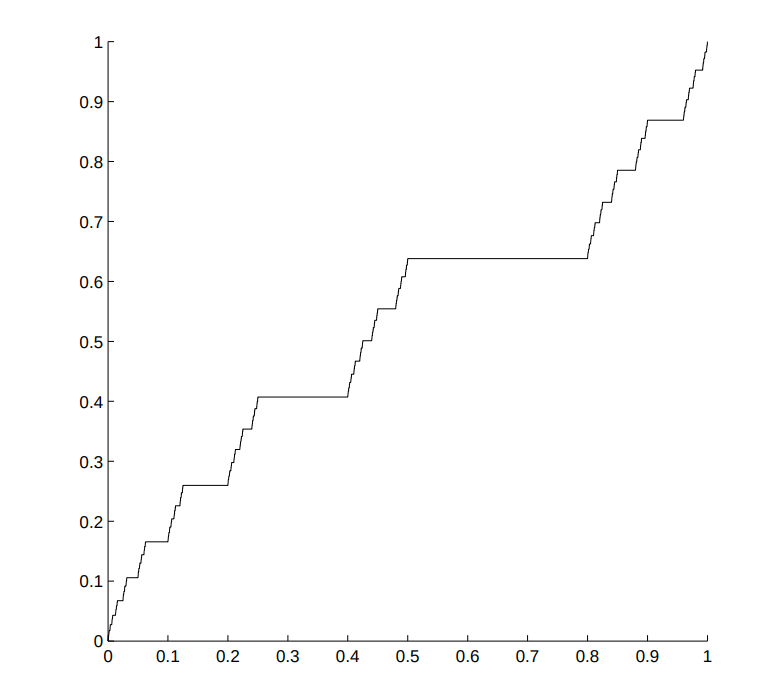
\includegraphics[width=0.7\textwidth]{chapters/chapter4/sections/plots/devils_staircase.png}
\end{center}

\textbf{Properties of the Cantor Function (CDF of \( X \))}\\

(a) It is \textbf{continuous everywhere} across \( [0, 1] \), meaning it has no jump discontinuities.\\
(b) Its derivative is \textbf{zero almost everywhere}, reflecting that the function has a flat slope at almost every point in \( [0, 1] \) except on the Cantor set itself.\\
(c) At points in the Cantor set \( C \), the function increases in value, yet it does so in a manner without a well-defined derivative at those points—illustrating its \textit{staircase} nature without abrupt jumps.\\

The Cantor function thus \textit{climbs} incrementally across the interval \( [0, 1] \) by increasing only at points in the Cantor set. This results in a singular CDF that is entirely smooth yet almost everywhere flat, a distinctive feature setting it apart from typical continuous or discrete distributions.


\begin{exercise}
    Consider a random variable \( X \). Prove that 

\[
P_X(\{y\}) = F_X(y) - \lim_{x \uparrow y} F_X(x).
\]

Furthermore, show that the cumulative distribution function \( F_X \) is continuous at the point \( y \) if and only if the probability that \( X \) takes the value \( y \), denoted as \( P_X(\{y\}) \), is equal to zero.
\end{exercise}

\begin{solution}
Let \( X \) be a random variable, and we want to prove the following statement: 

\[
P_X(\{y\}) = F_X(y) - \lim_{x \uparrow y} F_X(x)
\]

where \( F_X(y) \) denotes the cumulative distribution function (CDF) of \( X \), which is defined as 

\[
F_X(y) = P_X(X \leq y).
\]

To understand the left-hand side, \( P_X(\{y\}) \), we interpret it as the probability that the random variable \( X \) takes on the specific value \( y \). This can be thought of as the measure of the set \( \{y\} \) under the probability measure defined by \( X \).\\

Now, consider the right-hand side of the equation. The term \( F_X(y) \) represents the probability that \( X \) is less than or equal to \( y \). In contrast, \( \lim_{x \uparrow y} F_X(x) \) gives us the probability that \( X \) is less than \( y \) as we approach \( y \) from the left.\\

Thus, we can interpret the difference \( F_X(y) - \lim_{x \uparrow y} F_X(x) \) as the \textit{amount} of probability mass located precisely at \( y \). If there is a non-zero probability that \( X \) equals \( y \), then the CDF will increase at that point, resulting in a positive difference.\\

Next, we will show that \( F_X \) is continuous at \( y \) if and only if \( P_X(\{y\}) = 0 \). \\

(a) \textit{If \( F_X \) is continuous at \( y \)}:
\[
   \text{Then } \lim_{x \uparrow y} F_X(x) = F_X(y).
   \]
   Therefore,
   \[
   P_X(\{y\}) = F_X(y) - \lim_{x \uparrow y} F_X(x) = F_X(y) - F_X(y) = 0.
   \]

(b) \textit{Conversely, if \( P_X(\{y\}) = 0 \)}:
This implies that 
   \[
   F_X(y) - \lim_{x \uparrow y} F_X(x) = 0.
   \]
   Hence,
   \[
   F_X(y) = \lim_{x \uparrow y} F_X(x).
   \]
   This shows that \( F_X \) is continuous at \( y \).\\

In summary, we have established that \( P_X(\{y\}) = F_X(y) - \lim_{x \uparrow y} F_X(x) \), and that \( F_X \) is continuous at \( y \) if and only if \( P_X(\{y\}) = 0 \). \\
\end{solution}


\begin{exercise}
Among the functions given below, identify which are valid cumulative distribution functions (CDFs) and find their corresponding densities. For those that are not valid CDFs, explain the failures.

\textbf{(a) } 
\[
    F(x) = 
    \begin{cases} 
    1 - e^{-x^2} & x \geq 0 \\ 
    0 & x < 0 
    \end{cases}
\]


\textbf{(b) } 
\[
    F(x) = 
    \begin{cases} 
    e^{-\frac{1}{x}} & x > 0 \\ 
    0 & x \leq 0 
    \end{cases}
\]

\textbf{(c) } 
\[
    F(x) = 
    \begin{cases} 
    0 & x \leq 0 \\ 
    \frac{1}{3} & 0 < x \leq 1 \\ 
    2 & x > 1 
    \end{cases}
\]

\end{exercise}

\begin{solution}

\textbf{(a) Analysis:} \\

(a) For \( x < 0 \), \( F(x) = 0 \).\\
(b) For \( x \geq 0 \), as \( x \to 0 \), \( F(0) = 1 - e^{0} = 0 \), and as \( x \to \infty \), \( F(x) \to 1 \).\\
(c) The function is non-decreasing for \( x \geq 0 \) since the derivative \( F'(x) = 2x e^{-x^2} \) is non-negative.\\

Thus, \( F(x) \) is a valid CDF.\\

\textbf{Finding the Density:} The PDF is given by the derivative:
\[
f(x) = \frac{d}{dx}F(x) = 
\begin{cases} 
2x e^{-x^2} & x \geq 0 \\ 
0 & x < 0 
\end{cases}
\]

\textbf{(b) Analysis:} \\

(a) For \( x \leq 0 \), \( F(x) = 0 \).\\
(b) As \( x \to 0^+ \), \( F(x) \to 0 \), but as \( x \to \infty \), \( F(x) \to 1 \).\\
(c) However, the function is non-decreasing for \( x \geq 0 \) because the derivative \( F'(x) = e^{-\frac{1}{x}} \cdot \frac{1}{x^2} \) is always positive.\\

Thus, \( F(x) \) is a valid CDF.\\

\textbf{Finding the Density:} The PDF is given by the derivative:
\[
f(x) = \frac{d}{dx}F(x) = 
\begin{cases} 
    e^{-\frac{1}{x}} \cdot \frac{1}{x^2} & x \geq 0 \\ 
0 & x < 0 
\end{cases}
\]


\textbf{(c) Analysis:} \\

(a) For \( x \leq 0 \), \( F(x) = 0 \).\\
(b) For \( 0 < x \leq 1 \), \( F(x) = \frac{1}{3} \), which is constant and thus non-decreasing.\\
(c) However, for \( x > 1 \), \( F(x) = 2 \), which violates the upper limit condition of a CDF, as \( F(x) \) must approach \( 1 \) as \( x \to \infty \).\\

Thus, \( F(x) \) is not a valid CDF due to exceeding the limit of \( 1 \).\\


\end{solution}


\begin{exercise}
\textbf{Negative Binomial Random Variable.} Consider a sequence of independent Bernoulli trials \(\{X_i\}_{i \in \mathbb{N}}\) with parameter of success \(p \in (0, 1]\). The number of successes in the first \(n\) trials is given by 
\[
Y_n = \sum_{i=1}^{n} X_i.
\]
\(Y_n\) is distributed as Binomial with parameters \(n\) and \(p\). Consider the random variable defined by 
\[
V_k = \min\{n \in \mathbb{N}^+ : Y_n = k\}.
\]
Note that \(V_1\) is distributed as Geometric with parameter \(p\).\\

(a) Give a verbal description of the random variable \(V_k\)\\

(b) Show that the probability mass function of the random variable \(V_k\) is given by 
\[
P(V_k = n) = \binom{n-1}{k-1} p^k (1 - p)^{n-k},
\]
where \(n \in \{k, k + 1, \ldots\}\), we need to consider the conditions under which \(V_k = n\). \\

(c) Argue that the Binomial and Negative Binomial Distributions are inverse to each other in the sense that
\[
Y_n \geq k \Leftrightarrow V_k \leq n,
\]
\end{exercise}

\begin{solution}
\textbf{(a)} A verbal description of the random variable \(V_k\) is as follows: \(V_k\) represents the number of trials required to achieve exactly \(k\) successes in a series of independent Bernoulli trials, where each trial has a success probability of \(p\). In simpler terms, \(V_k\) tells us how many attempts we need to make until we obtain \(k\) successful outcomes.\\

\textbf{(b)} For \(V_k\) to equal \(n\), the following must hold:\\

1. The \(n\)-th trial must result in a success, contributing to the \(k\)-th success.\\
2. Among the first \(n-1\) trials, exactly \(k-1\) must be successes, ensuring that the \(k\)-th success occurs on the \(n\)-th trial.\\

The number of ways to select which \(k-1\) trials out of the first \(n-1\) are successful is given by \(\binom{n-1}{k-1}\). The probability of exactly \(k-1\) successes and \(n-k\) failures in the first \(n-1\) trials is given by \(p^{k-1} (1 - p)^{(n-1) - (k-1)}\) or \(p^{k-1} (1 - p)^{n-k}\). Finally, the \(n\)-th trial must be a success, contributing a factor of \(p\). Therefore, the total probability is:
\[
P(V_k = n) = \binom{n-1}{k-1} p^{k} (1 - p)^{n-k}.
\]

This is known as the Negative Binomial Distribution with parameters \(k\) and \(p\).\\

\textbf{(c)} To argue that the Binomial and Negative Binomial Distributions are inverse to each other in the sense that
\[
Y_n \geq k \Leftrightarrow V_k \leq n,
\]
we interpret these statements as follows:\\

(a) \(Y_n \geq k\) means that in \(n\) trials, we have at least \(k\) successes. This implies that the \(k\)-th success can occur at or before the \(n\)-th trial.\\

(b) \(V_k \leq n\) means that the \(k\)-th success occurs within the first \(n\) trials. This is equivalent to stating that we need \(n\) or fewer trials to achieve \(k\) successes.\\

Thus, the two statements describe the same event: having \(k\) successes in at most \(n\) trials. Consequently, we can conclude that \(Y_n \geq k \Leftrightarrow V_k \leq n\).\\
\end{solution}


\begin{exercise}
    Radioactive decay. Assume that a radioactive sample emits a random number of \(\alpha\) particles in any given hour, and that the number of \(\alpha\) particles emitted in an hour is Poisson distributed with parameter \(\lambda\). Suppose that a faulty Geiger-Muller counter is used to count these particle emissions. In particular, the faulty counter fails to register an emission with probability \(p\), independently of other emissions. \\

    (a) What is the probability that the faulty counter will register exactly \(k\) emissions in an hour? \\
    (b) Given that the faulty counter registered \(k\) emissions in an hour, what is the PMF of the actual number of emissions that happened from the source during that hour?
    \end{exercise}
    
    \begin{solution}
    To solve this problem, we will consider the nature of radioactive decay and the behavior of the faulty counter.\\
    
    First, we know that the number of \(\alpha\) particles emitted in an hour, denoted as \(X\), follows a Poisson distribution with parameter \(\lambda\):
    \[
    P(X = n) = \frac{\lambda^n e^{-\lambda}}{n!}
    \]
    for \(n = 0, 1, 2, \ldots\).\\
    
    The faulty counter registers an emission with probability \(1 - p\) and fails to register it with probability \(p\). Therefore, if \(X\) is the actual number of emissions, the number of emissions registered by the counter, denoted as \(Y\), follows a Binomial distribution:
    \[
    Y | X = n \sim \text{Binomial}(n, 1 - p).
    \]
    
    \textbf{(a)} We want to find the probability that the faulty counter registers exactly \(k\) emissions in an hour, which can be expressed as:
    \[
    P(Y = k) = \sum_{n=k}^{\infty} P(Y = k | X = n) P(X = n).
    \]
    
    The conditional probability \(P(Y = k | X = n)\) for the Binomial distribution is given by:
    \[
    P(Y = k | X = n) = \binom{n}{k} (1 - p)^k p^{n - k}.
    \]
    
    Thus, we have:
    \[
    P(Y = k) = \sum_{n=k}^{\infty} \binom{n}{k} (1 - p)^k p^{n - k} \frac{\lambda^n e^{-\lambda}}{n!}.
    \]
    
    This can be simplified by recognizing that:
    \[
    \binom{n}{k} \frac{1}{n!} = \frac{1}{k!(n-k)!}.
    \]
    
    The expression for \(P(Y = k)\) becomes:
    \[
    P(Y = k) = (1 - p)^k \frac{1}{k!} \sum_{n=k}^{\infty} \frac{(\lambda p)^{n - k}}{(n - k)!} e^{-\lambda}.
    \]
    The inner sum is the series expansion for the exponential function, leading to:
    \[
    \sum_{m=0}^{\infty} \frac{(\lambda p)^m}{m!} = e^{\lambda p}.
    \]
    Therefore, we obtain:
    \[
    P(Y = k) = (1 - p)^k \frac{(\lambda (1 - p))^k e^{-\lambda}}{k!}.
    \]
    
    This shows that \(Y\) also follows a Poisson distribution with parameter \(\lambda (1 - p)\):
    \[
    P(Y = k) = \frac{(\lambda (1 - p))^k e^{-\lambda (1 - p)}}{k!}.
    \]
    
    \textbf{(b)} Next, we need to find the PMF of the actual number of emissions \(X\) given that the counter registered \(k\) emissions:
    \[
    P(X = n | Y = k).
    \]
    Using Bayes' theorem, we can express this as:
    \[
    P(X = n | Y = k) = \frac{P(Y = k | X = n) P(X = n)}{P(Y = k)}.
    \]
    
    Substituting the earlier expressions, we find:
    \[
    P(X = n | Y = k) = \frac{\binom{n}{k} (1 - p)^k p^{n - k} \frac{\lambda^n e^{-\lambda}}{n!}}{P(Y = k)}.
    \]
    
    Given that \(P(Y = k)\) has already been derived, we can substitute this back into our equation. This results in a formula that allows us to compute the conditional probabilities depending on the values of \(n\) and \(k\).\\
    
    In summary, the solution outlines the Poisson nature of emissions and the impact of a faulty counter on the observed counts. 
    \end{solution}
    


\begin{exercise}
Buses arrive at ten minute intervals starting at noon. A man arrives at the bus stop at a random time \(X\) minutes after noon, where \(X\) has the CDF:
\[
F_X(x) =
\begin{cases}
0 & x < 0 \\
\frac{x}{60} & 0 \leq x \leq 60 \\
1 & x > 60.
\end{cases}
\]
What is the probability that he waits less than five minutes for a bus?
\end{exercise}

\begin{solution}
To solve this problem, we first need to understand the situation described. The man arrives at the bus stop at a random time \(X\) uniformly distributed between 0 and 60 minutes after noon. The buses arrive every 10 minutes, which means they arrive at 0, 10, 20, 30, 40, 50, and 60 minutes. The key is to find the probability that the man waits less than 5 minutes for the next bus.\\

The waiting time \(W\) can be calculated based on when he arrives at the bus stop:\\

1. If \(X \in [0, 5)\), the wait time \(W < 5\).\\
2. If \(X \in [5, 10)\), then \(W = 10 - X < 5\) corresponds to \(X > 5\), which means he waits for 0 to 5 minutes.\\
3. This pattern continues for \(X \in [10, 15)\), where he will again have a wait time of less than 5 minutes.\\

More formally, we can analyze the intervals for which \(W < 5\): \(X\) in the intervals \([0, 5)\) and \([10, 15)\), and so on up to \([50, 55)\).\\

To summarize the intervals where \(W < 5\):
\[
X \in [0, 5) \cup [10, 15) \cup [20, 25) \cup [30, 35) \cup [40, 45) \cup [50, 55).
\]

Thus, the total length of intervals where the man waits less than 5 minutes is:
\[
6 \times 5 = 30 \text{ minutes}.
\]

Since \(X\) is uniformly distributed over the interval \([0, 60]\), the probability \(P(W < 5)\) is the ratio of the total length of intervals where he waits less than 5 minutes to the total possible time (60 minutes):
\[
P(W < 5) = \frac{30}{60} = \frac{1}{2}.
\]
\end{solution}


\begin{exercise}
Find the values of \( a \) and \( b \) such that the following function is a valid CDF:
\[
F(x) = 
\begin{cases}
1 - ae^{-x/b} & \text{for } x \geq 0 \\
0 & \text{for } x < 0
\end{cases}
\]
Also, find the values of \( a \) and \( b \) such that the function above corresponds to the CDF of some:
\begin{enumerate}
    \item Continuous Random Variable
    \item Discrete Random Variable
    \item Mixed type Random Variable
\end{enumerate}
\end{exercise}

\begin{solution}
To determine the values of \( a \) and \( b \) that make \( F(x) \) a valid cumulative distribution function (CDF), we need to ensure that:\\

1. \( F(x) \) is non-decreasing.\\
2. \( \lim_{x \to -\infty} F(x) = 0 \) and \( \lim_{x \to \infty} F(x) = 1 \).\\

For the given function \( F(x) \):\\

1. For \( x < 0 \), we have \( F(x) = 0 \), which satisfies the first condition.\\
2. For \( x \geq 0 \), we have \( F(x) = 1 - ae^{-x/b} \).\\

Next, we examine the limits:\\

(a) As \( x \to 0 \):
\[
F(0) = 1 - ae^{0} = 1 - a
\]
To ensure that \( F(0) \) is non-negative, we require:
\[
1 - a \geq 0 \implies a \leq 1
\]

(b) As \( x \to \infty \):
\[
F(x) \to 1 - a \cdot 0 = 1
\]
This is valid if \( a > 0 \) to ensure \( F(x) \) approaches 1 correctly.\\

Thus, from these conditions, we have:
\[
0 < a \leq 1
\]

Next, for \( b \), the exponential function \( e^{-x/b} \) is defined for all \( x \) when \( b > 0 \). Therefore, we must have:
\[
b > 0
\]

In summary, the parameters \( a \) and \( b \) must satisfy:
\[
0 < a \leq 1 \\
b > 0
\]

Now, let’s analyze the types of random variables.\\

(a) \textit{Continuous Random Variable}\\

For \( F(x) \) to represent the CDF of a continuous random variable, the function \( F(x) \) must be strictly increasing. This requires:
\[
a > 0 \quad \text{and} \quad b > 0
\]
Therefore, the same conditions hold.\\

(b) \textit{Discrete Random Variable}\\

For a discrete random variable, \( F(x) \) should have jumps at specific values. In this case, we can choose \( a = 1 \) and \( b \) can be any positive number. Thus:
\[
a = 1, \quad b > 0
\]

(c) \textit{Mixed Random Variable}\\

For a mixed type random variable, \( F(x) \) must be a combination of both continuous and discrete. We can choose \( a < 1 \) and \( b > 0 \). This allows \( F(x) \) to have a continuous component as well as a discrete one at \( x = 0 \). Thus, we can set:
\[
0 < a < 1, \quad b > 0
\]

\end{solution}

    

\begin{exercise}
Let \( X \) be a continuous random variable. Show that \( X \) is memoryless if and only if \( X \) is an exponential random variable.
\end{exercise}

\begin{solution}
To demonstrate that a continuous random variable \( X \) is memoryless if and only if it is an exponential random variable, we first define what it means for \( X \) to be memoryless. A random variable \( X \) is said to be memoryless if it satisfies the following condition for all \( s, t \geq 0 \):

\[
P(X > s + t \mid X > s) = P(X > t).
\]

This equation states that the probability that \( X \) exceeds \( s + t \), given that it has already exceeded \( s \), is the same as the probability that \( X \) exceeds \( t \) alone. \\

(\(\Rightarrow\)) We begin by assuming that \( X \) is memoryless. To show that \( X \) is an exponential random variable, we will derive its cumulative distribution function (CDF) and probability density function (PDF).\\

Let \( F(x) = P(X \leq x) \) be the CDF of \( X \). Consequently, the survival function, which gives the probability that \( X \) exceeds \( x \), is:

\[
S(x) = P(X > x) = 1 - F(x).
\]

Now, using the memoryless property, we have:

\[
P(X > s + t \mid X > s) = \frac{P(X > s + t)}{P(X > s)}.
\]

Using the memoryless condition, we equate this to \( P(X > t) \):

\[
\frac{S(s+t)}{S(s)} = S(t).
\]

Rearranging gives us:

\[
S(s + t) = S(s) S(t).
\]

This functional equation resembles the form of the survival function of an exponential distribution. If we denote \( S(t) = e^{-\lambda t} \) for some \( \lambda > 0 \), then we can verify that:

\[
S(s+t) = e^{-\lambda (s+t)} = e^{-\lambda s} e^{-\lambda t} = S(s) S(t).
\]

Thus, \( S(t) \) takes the form of the exponential survival function, confirming that \( X \) is indeed an exponential random variable.\\

(\(\Leftarrow\)) Conversely, suppose that \( X \) is an exponential random variable with parameter \( \lambda \). The survival function is given by:

\[
S(t) = P(X > t) = e^{-\lambda t}.
\]

We can apply this to check the memoryless property:

\[
P(X > s + t \mid X > s) = \frac{P(X > s+t)}{P(X > s)} = \frac{e^{-\lambda (s+t)}}{e^{-\lambda s}} = e^{-\lambda t} = P(X > t).
\]

Since this holds for all \( s, t \geq 0 \), we conclude that the exponential distribution satisfies the memoryless property.\\

In summary, we have shown that \( X \) is memoryless if and only if \( X \) is an exponential random variable.
\end{solution}
